\subsection{消毒池}
\subsubsection{消毒方式的选择}

臭氧由3个氧原子组成,极不稳定,分解时产生初生态氧[O],具有极强的氧化能力,是除氟以外最活泼的氧化剂,对具有极强抵抗力的微生物如病毒、芽孢等具有很强的杀伤力。[O]还有很强的渗入细胞壁的能力,从而破坏细菌有机链状结构导致细菌的死亡。臭氧消毒的一般工艺流程如图  所示。

\begin{figure}[H]
	\centering
	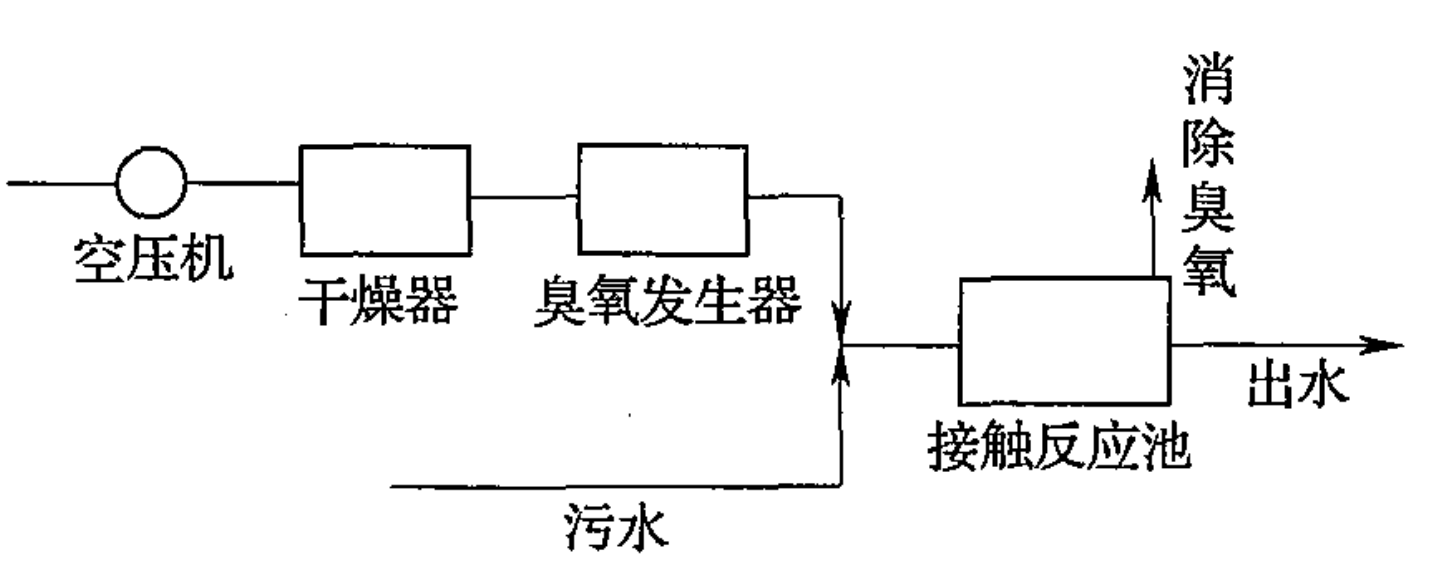
\includegraphics[width=0.6\textwidth]{figures/Ozone disinfection process.png}
	\caption{臭氧消毒流程\cite[p.387]{《第2册排水工程》}}
	\label{fig:Ozone disinfection process}
\end{figure}

臭氧在水中的溶解度仅为 10 mg/L左右,因此通人污水中的臭氧往往不可能全部被利用,为了提高臭氧的利用率,接触反应池最好建成水深为 $4\sim 6$ m的深水池,或建成封闭的几格串联的接触池,用管式或板式微孔扩散器扩散臭氧。臭氧消毒迅速,接触时间可采用15 min,能够维持的剩余臭氧量为 0.4 mg/L。接触池排出的剩余臭氧,具有腐蚀性,因此需作尾气破坏处理。臭氧不能贮存,需现场边发生边使用。臭氧消毒具有如下特点:
\begin{enumerate}
    \item 反应快,投量少,在水中不产生持久性残余,无二次污染;
    \item 适应能力强,在 $\text{pH} = 5.6 \sim 9.8$,水温 $0\sim 35$ ℃范围内,消毒性能稳定;
    \item 臭氧没有氯那样的持续消毒作用。
\end{enumerate}


\subsubsection{臭氧消毒接触池设计}

\begin{figure}[H]
	\centering
	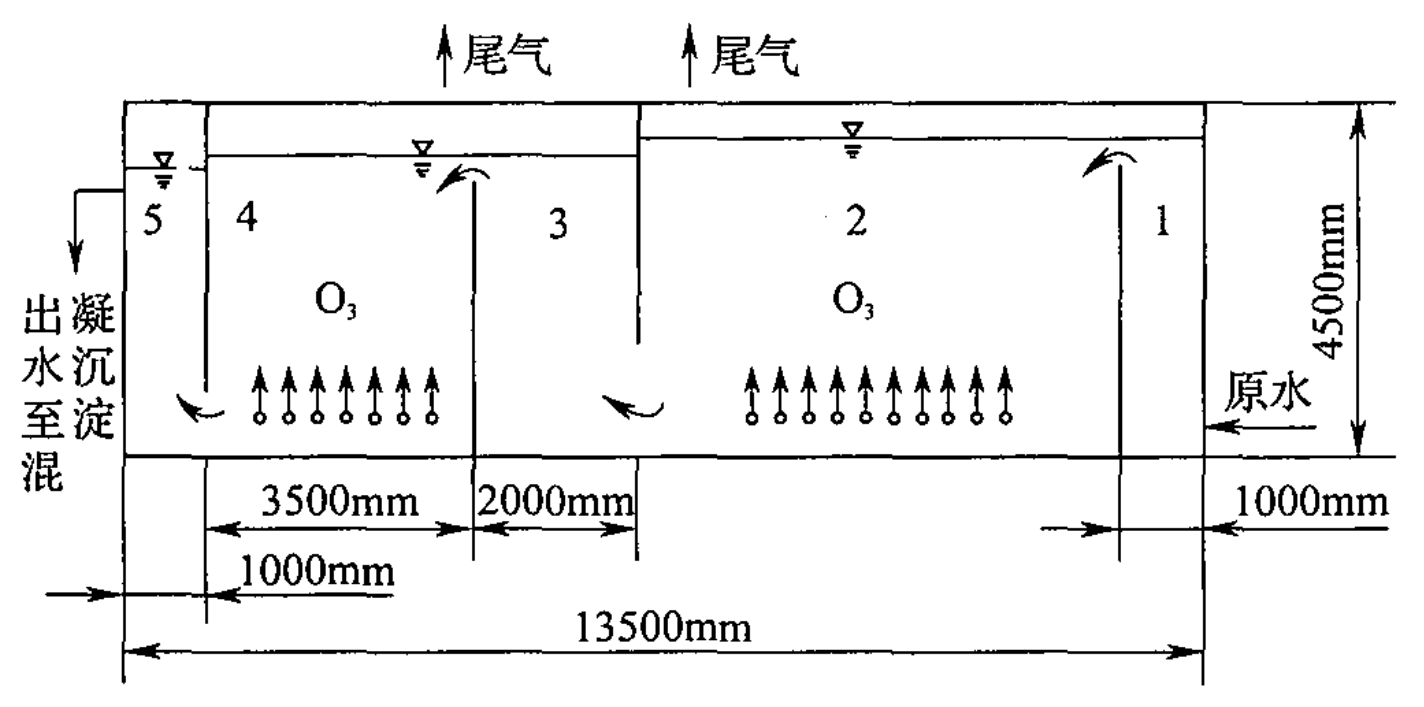
\includegraphics[width=0.8\textwidth]{figures/Ozone contact cell.png}
	\caption{臭氧接触池\cite[p.388]{《第2册排水工程》}}
	\label{fig:Ozone contact cell}
\end{figure}

\begin{enumerate}
	\item 容积
	
	\begin{equation}
		V=\dfrac{QT}{60}
	\end{equation}
	$V$——接触池容积,m$^3$;\par
	$Q$——所需消毒的污水流量,m$^3$/h;\par
	$T$——水力停留时间,mln,一般取 $5\sim 15$ min。

	因为 $Q_{max}=58100 \;\text{m$^3$/d}$ ,取水力停留时间 $T=9$ min ,则臭氧消毒接触池容积为
	\begin{align*}
		V = \dfrac{Q_{max}T}{60} = \dfrac{58100\times 9}{60\times 24} \;\text{m$^3$} = \eval{\dfrac{58100\times 9}{60\times 24}} \;\text{m$^3$} 
	\end{align*}

	\item 尺寸设计
	
	设池宽为 6 m ,其余尺寸如图 \ref{fig:Ozone contact cell} 所示,则其容积为
	\begin{align}
		V &= 6 \times 4.5 \times 13.5 \;\text{m$^3$} = \eval{6 \times 4.5 \times 13.5} \;\text{m$^3$} \\
		& > 363.125 \;\text{m$^3$(满足有效停留时间要求)} \notag
	\end{align}

	\item 1、3、5室的水流速度 $v_1$、$v_3$、$v_5$ 计算
	
	\begin{align}
		v_1 = v_5 = \dfrac{58100}{24}\times \dfrac{10^2}{3600\times 6\times 1.0} \;\text{cm/s} = \eval{\dfrac{58100}{24}\times \dfrac{10^2}{3600\times 6\times 1.0}}[3] \;\text{cm/s}
	\end{align}
	\begin{align}
		v_3 = \dfrac{1}{2}v_1 = \eval{\dfrac{11.208}{2}} \;\text{cm/s}
	\end{align}
\end{enumerate}


\subsubsection{臭氧发生器所需空气量}
\begin{enumerate}
	\item 臭氧需要量
	
	\begin{equation}
		D = 1.06\alpha Q 
	\end{equation}
	$D$——臭氧需要量,g/h;\par
	$\alpha$——臭氧投加量 g/m$^3$;\par
	$1.06$——安全系数;\par
	$Q$——所需消毒的污水流量,m$^3$/h。

	取最大投加臭氧量 $\alpha=2$ g/m$^3$,则臭氧需要量为
	\begin{align*}
		D = 1.06\alpha Q_{max} = 1.06\times 2 \times \dfrac{58100}{24} \;\text{g/h} = \eval{1.06\times 2 \times \dfrac{58100}{24}}[3] \;\text{g/h}
	\end{align*}

	\item 臭氧化所需空气量
	
	取臭氧化空气的臭氧含量 $c=10$ g/m$^3$,则臭氧化所需空气量为
	\begin{equation}
		V_{\text{干}} = \dfrac{D}{c} = \dfrac{5132.167}{10} \;\text{m$^3$/h} = \eval{\dfrac{5132.167}{10}} \;\text{m$^3$/h}
	\end{equation}
\end{enumerate}

